\documentclass[spanish, fleqn]{standalone}
\usepackage{babel}
\usepackage{tikz}
\usepackage{pgfplots}
\pgfplotsset{compat = 1.16}

\usetikzlibrary{arrows}

\begin{document}
  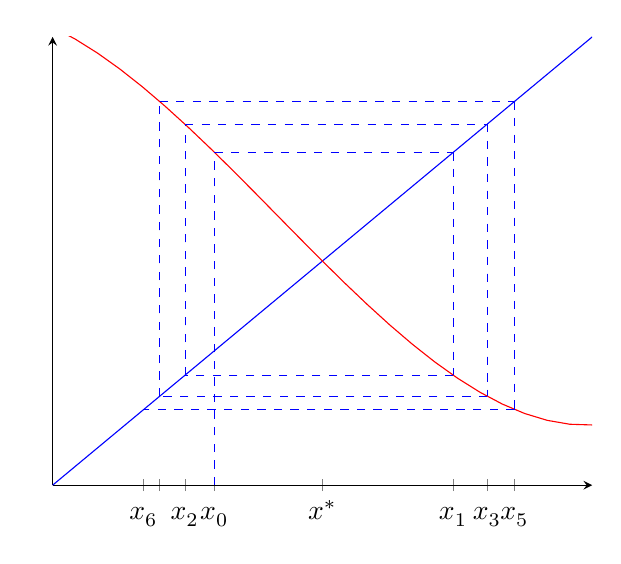
\begin{tikzpicture}
    \begin{axis}[domain = 0:1,
                 axis x line = bottom, axis y line = left,
                 xmin = 0, xmax = 1,
                 ymin = 0, ymax = 1,
                 xtick = {0.3, 0.7425, 0.245202598, 0.8053675633204307, 0.19829350349601982, 0.8561644490113705, 0.1687199716882174, 0.5},
                 xticklabels = {\(x_0^{\phantom{\ast}}\),
                                \(x_1^{\phantom{\ast}}\),
                                \(x_2^{\phantom{\ast}}\),
                                \(x_3^{\phantom{\ast}}\),
                                \(\),
                                \(x_5^{\phantom{\ast}}\),
                                \(x_6^{\phantom{\ast}}\),
                                \(x^{\ast}_{\phantom{0}}\)},
                 ytick style = {draw = none},
                 yticklabels = {}]

      \addplot[mark = none, blue] {x};
      \addplot[mark = none, red]
        {5 * x^3 / 4 - 25 * x^2 / 16 - 23 * x / 40 + 327 / 320};

    \draw [blue, very thin, dashed]
       (axis cs:0.3, 0) -- (axis cs:0.3, 0.7425);
    \draw [blue, very thin, dashed]
       (axis cs:0.3, 0.7425) -- (axis cs:0.7425, 0.7425);
    \draw [blue, very thin, dashed]
       (axis cs:0.7425, 0.7425) -- (axis cs:0.7425, 0.245202598);
    \draw [blue, very thin, dashed]
       (axis cs:0.7425, 0.245202598) -- (axis cs:0.245202598, 0.245202598);
    \draw [blue, very thin, dashed]
       (axis cs:0.245202598, 0.245202598) -- (axis cs:0.245202598, 0.8053675633204307);
    \draw [blue, very thin, dashed]
       (axis cs:0.245202598, 0.245202598) -- (axis cs:0.245202598, 0.8053675633204307);
    \draw [blue, very thin, dashed]
       (axis cs:0.245202598, 0.8053675633204307) -- (axis cs:0.8053675633204307, 0.8053675633204307);
    \draw [blue, very thin, dashed]
       (axis cs:0.8053675633204307, 0.8053675633204307) -- (axis cs:0.8053675633204307, 0.19829350349601982);
    \draw [blue, very thin, dashed]
       (axis cs:0.8053675633204307, 0.8053675633204307) -- (axis cs:0.8053675633204307, 0.19829350349601982);
    \draw [blue, very thin, dashed]
       (axis cs:0.8053675633204307, 0.19829350349601982) -- (axis cs:0.19829350349601982, 0.19829350349601982);
    \draw [blue, very thin, dashed]
       (axis cs:0.19829350349601982, 0.19829350349601982) -- (axis cs:0.19829350349601982, 0.8561644490113705);
    \draw [blue, very thin, dashed]
       (axis cs:0.19829350349601982, 0.19829350349601982) -- (axis cs:0.19829350349601982, 0.8561644490113705);
    \draw [blue, very thin, dashed]
       (axis cs:0.19829350349601982, 0.8561644490113705) -- (axis cs:0.8561644490113705, 0.8561644490113705);
    \draw [blue, very thin, dashed]
       (axis cs:0.8561644490113705, 0.8561644490113705) -- (axis cs:0.8561644490113705, 0.1687199716882174);
    \draw [blue, very thin, dashed]
       (axis cs:0.8561644490113705, 0.1687199716882174) -- (axis cs:0.1687199716882174, 0.1687199716882174);
    \end{axis}
  \end{tikzpicture}
\end{document}
